\documentclass[]{book}
\usepackage{lmodern}
\usepackage{amssymb,amsmath}
\usepackage{ifxetex,ifluatex}
\usepackage{fixltx2e} % provides \textsubscript
\ifnum 0\ifxetex 1\fi\ifluatex 1\fi=0 % if pdftex
  \usepackage[T1]{fontenc}
  \usepackage[utf8]{inputenc}
\else % if luatex or xelatex
  \ifxetex
    \usepackage{mathspec}
  \else
    \usepackage{fontspec}
  \fi
  \defaultfontfeatures{Ligatures=TeX,Scale=MatchLowercase}
\fi
% use upquote if available, for straight quotes in verbatim environments
\IfFileExists{upquote.sty}{\usepackage{upquote}}{}
% use microtype if available
\IfFileExists{microtype.sty}{%
\usepackage{microtype}
\UseMicrotypeSet[protrusion]{basicmath} % disable protrusion for tt fonts
}{}
\usepackage[margin=1in]{geometry}
\usepackage{hyperref}
\hypersetup{unicode=true,
            pdftitle={Modeling Melodic Dictation},
            pdfauthor={David John Baker},
            pdfborder={0 0 0},
            breaklinks=true}
\urlstyle{same}  % don't use monospace font for urls
\usepackage{natbib}
\bibliographystyle{apalike}
\usepackage{color}
\usepackage{fancyvrb}
\newcommand{\VerbBar}{|}
\newcommand{\VERB}{\Verb[commandchars=\\\{\}]}
\DefineVerbatimEnvironment{Highlighting}{Verbatim}{commandchars=\\\{\}}
% Add ',fontsize=\small' for more characters per line
\usepackage{framed}
\definecolor{shadecolor}{RGB}{248,248,248}
\newenvironment{Shaded}{\begin{snugshade}}{\end{snugshade}}
\newcommand{\AlertTok}[1]{\textcolor[rgb]{0.94,0.16,0.16}{#1}}
\newcommand{\AnnotationTok}[1]{\textcolor[rgb]{0.56,0.35,0.01}{\textbf{\textit{#1}}}}
\newcommand{\AttributeTok}[1]{\textcolor[rgb]{0.77,0.63,0.00}{#1}}
\newcommand{\BaseNTok}[1]{\textcolor[rgb]{0.00,0.00,0.81}{#1}}
\newcommand{\BuiltInTok}[1]{#1}
\newcommand{\CharTok}[1]{\textcolor[rgb]{0.31,0.60,0.02}{#1}}
\newcommand{\CommentTok}[1]{\textcolor[rgb]{0.56,0.35,0.01}{\textit{#1}}}
\newcommand{\CommentVarTok}[1]{\textcolor[rgb]{0.56,0.35,0.01}{\textbf{\textit{#1}}}}
\newcommand{\ConstantTok}[1]{\textcolor[rgb]{0.00,0.00,0.00}{#1}}
\newcommand{\ControlFlowTok}[1]{\textcolor[rgb]{0.13,0.29,0.53}{\textbf{#1}}}
\newcommand{\DataTypeTok}[1]{\textcolor[rgb]{0.13,0.29,0.53}{#1}}
\newcommand{\DecValTok}[1]{\textcolor[rgb]{0.00,0.00,0.81}{#1}}
\newcommand{\DocumentationTok}[1]{\textcolor[rgb]{0.56,0.35,0.01}{\textbf{\textit{#1}}}}
\newcommand{\ErrorTok}[1]{\textcolor[rgb]{0.64,0.00,0.00}{\textbf{#1}}}
\newcommand{\ExtensionTok}[1]{#1}
\newcommand{\FloatTok}[1]{\textcolor[rgb]{0.00,0.00,0.81}{#1}}
\newcommand{\FunctionTok}[1]{\textcolor[rgb]{0.00,0.00,0.00}{#1}}
\newcommand{\ImportTok}[1]{#1}
\newcommand{\InformationTok}[1]{\textcolor[rgb]{0.56,0.35,0.01}{\textbf{\textit{#1}}}}
\newcommand{\KeywordTok}[1]{\textcolor[rgb]{0.13,0.29,0.53}{\textbf{#1}}}
\newcommand{\NormalTok}[1]{#1}
\newcommand{\OperatorTok}[1]{\textcolor[rgb]{0.81,0.36,0.00}{\textbf{#1}}}
\newcommand{\OtherTok}[1]{\textcolor[rgb]{0.56,0.35,0.01}{#1}}
\newcommand{\PreprocessorTok}[1]{\textcolor[rgb]{0.56,0.35,0.01}{\textit{#1}}}
\newcommand{\RegionMarkerTok}[1]{#1}
\newcommand{\SpecialCharTok}[1]{\textcolor[rgb]{0.00,0.00,0.00}{#1}}
\newcommand{\SpecialStringTok}[1]{\textcolor[rgb]{0.31,0.60,0.02}{#1}}
\newcommand{\StringTok}[1]{\textcolor[rgb]{0.31,0.60,0.02}{#1}}
\newcommand{\VariableTok}[1]{\textcolor[rgb]{0.00,0.00,0.00}{#1}}
\newcommand{\VerbatimStringTok}[1]{\textcolor[rgb]{0.31,0.60,0.02}{#1}}
\newcommand{\WarningTok}[1]{\textcolor[rgb]{0.56,0.35,0.01}{\textbf{\textit{#1}}}}
\usepackage{longtable,booktabs}
\usepackage{graphicx,grffile}
\makeatletter
\def\maxwidth{\ifdim\Gin@nat@width>\linewidth\linewidth\else\Gin@nat@width\fi}
\def\maxheight{\ifdim\Gin@nat@height>\textheight\textheight\else\Gin@nat@height\fi}
\makeatother
% Scale images if necessary, so that they will not overflow the page
% margins by default, and it is still possible to overwrite the defaults
% using explicit options in \includegraphics[width, height, ...]{}
\setkeys{Gin}{width=\maxwidth,height=\maxheight,keepaspectratio}
\IfFileExists{parskip.sty}{%
\usepackage{parskip}
}{% else
\setlength{\parindent}{0pt}
\setlength{\parskip}{6pt plus 2pt minus 1pt}
}
\setlength{\emergencystretch}{3em}  % prevent overfull lines
\providecommand{\tightlist}{%
  \setlength{\itemsep}{0pt}\setlength{\parskip}{0pt}}
\setcounter{secnumdepth}{5}
% Redefines (sub)paragraphs to behave more like sections
\ifx\paragraph\undefined\else
\let\oldparagraph\paragraph
\renewcommand{\paragraph}[1]{\oldparagraph{#1}\mbox{}}
\fi
\ifx\subparagraph\undefined\else
\let\oldsubparagraph\subparagraph
\renewcommand{\subparagraph}[1]{\oldsubparagraph{#1}\mbox{}}
\fi

%%% Use protect on footnotes to avoid problems with footnotes in titles
\let\rmarkdownfootnote\footnote%
\def\footnote{\protect\rmarkdownfootnote}

%%% Change title format to be more compact
\usepackage{titling}

% Create subtitle command for use in maketitle
\newcommand{\subtitle}[1]{
  \posttitle{
    \begin{center}\large#1\end{center}
    }
}

\setlength{\droptitle}{-2em}
  \title{Modeling Melodic Dictation}
  \pretitle{\vspace{\droptitle}\centering\huge}
  \posttitle{\par}
  \author{David John Baker}
  \preauthor{\centering\large\emph}
  \postauthor{\par}
  \predate{\centering\large\emph}
  \postdate{\par}
  \date{2018-08-27}

\usepackage{booktabs}
\usepackage{amsthm}
\makeatletter
\def\thm@space@setup{%
  \thm@preskip=8pt plus 2pt minus 4pt
  \thm@postskip=\thm@preskip
}
\makeatother

\usepackage{amsthm}
\newtheorem{theorem}{Theorem}[chapter]
\newtheorem{lemma}{Lemma}[chapter]
\theoremstyle{definition}
\newtheorem{definition}{Definition}[chapter]
\newtheorem{corollary}{Corollary}[chapter]
\newtheorem{proposition}{Proposition}[chapter]
\theoremstyle{definition}
\newtheorem{example}{Example}[chapter]
\theoremstyle{definition}
\newtheorem{exercise}{Exercise}[chapter]
\theoremstyle{remark}
\newtheorem*{remark}{Remark}
\newtheorem*{solution}{Solution}
\begin{document}
\maketitle

{
\setcounter{tocdepth}{1}
\tableofcontents
}
\hypertarget{significance-of-the-study}{%
\chapter{Significance of the Study}\label{significance-of-the-study}}

All students pursing a Bachelor's degree in Music from universities
accredited by the National Association of Schools of Music must learn to
take melodic dictation \citep[ Section
VIII.6.B.2.A]{NationalAssociationSchools2018}. Melodic dictation is a
cognitively demanding process that requires students to listen to a
melody, retain it in memory, and then use their knowledge of Western
musical notation in order to recreate the mental image of the melody on
paper in a limited time frame. As of 2018 there are 647 Schools of Music
belonging to National Association of Schools of Music (NASM) CITE
WEBSITE, meaning that hundereds of students every year will be expected
to learn this challenging task as part of their Aural Skills education.
The logic being that as one improves in their abiliy to take melodic
dictation, this practice of critical and active listening develops as a
means to improve one's ability to ``think in music'' and thus become a
more compotent musician. While learning Aural Skills has been a hallmark
of being educated within the Western conservatory tradition, the
rationale behind both the how and why of aural skills is often thought
of as being esoteric. Throughout the past century, people have disagreed
on exactly how one does go about learning a melody with different areas
of research each attacking the problem from a different angle.

Despite its ubiqiquity in curricula within School of Music settings,
research on topics pertain to how aural skills are acquired is limited
at best. The fields of music theory and cognitive psychology are best
positioned to make progress on this question, but often the skills
required to be well versed ein ither of these subjects are disparate,
published in other journals, and the research with overlap is scarce.
This problem is not new and there have been repeated attempts to bridge
the gap between practioners of aural skills and people in cognitive
psycholgy CITES. Literature from music theory has establisehd conceptual
frameworks regarding aural skills
\citet{karpinskiAuralSkillsAcquisition2000} and the relavint cognitive
psychology literature has explored factors that might contribute to
melodic perception (SCHMUKLER SYNERR 2016 2016), and there exists
applied literature from the world of music education (CITES).

However, despite these siloed areas of research, we as music researchers
do not have an a concrete understanding of exaclty what contributes to
HOW individuals learn melodies (HALPERNBARLETT2010). This is peculiar
since ``how does one learn a melody'' seems to be one of the fundamental
questions to the fields of music theory, music psychology, as well as
music education. Given this lack of understanding, it becomes even more
peculiar that this lack of convergence of evidence is then unable to
provide a solid baseline as to what student in their aural skills
classrooms can be expected to do. (Also something about we should really
know this if we are going to grade people on this ability). While no
single dissertation can solve any problem completely, this dissertation
aims to fill the gap in the literature between aural skills
practitioners (theorists and educators) and music psychologists in order
to reach conclusion that can be applied systematically in pedagogical
contexts. In order to do this I draw both literatures (music and
science) in order to demonstrate how tools from both cognitive
psychology as well as computational musicology can help move both fields
forward. Some line here about if we really want to understand what is
happening we need to know about causal factors going on here and have
experimental manipulation and things like making models of the whole
thing. Great to rely on some sort of anecdoatal evidence, but if we are
going to put things on the line with our education then we need to be
able to make some sort of falsifiable claims about what we are doing.
Can only do that through the lens of science.

\hypertarget{chapter-overview}{%
\section{Chapter Overview}\label{chapter-overview}}

In this first chapter, I introduce the process of melodic dictation and
discuss factors that would presumably could play a role in taking
melodic dictation. The chapter introduces both a theoretical backgorund
and rationale for using method form both computational musicology and
congitive psychology in order ot answr quesitona bout how individuals
learn melodies. I argue that tools for understanding this best because
as we currently understand it, I see us operating in a Kuhnian normal
science where much can be learned by just using the tools in front of
us. This chapter will clearly outline the factors hypothesized to
contribute to an individual's abilit to learn melodies, incorporating
both individual and musical parameters. The chapter ends with a
discussion some of the philosophical/theoretical problems with
attempting to measure thigns like this (is it just a party trick?) and
establishes that I will be taking a more polymorphic view of
musicianship in order to answer this question.

The second chapter of my dissertation focuses on the history and current
state of aural skills pedagogy.

Tracing back its origins to the practical need to teach musical skills
back with Guido d'Arezzo, I compare and contrast the different
methodological approaches that have been used, along with their goals.

The third chapter discusses previous work that examines individual
factors thought to contribute to one's ability to perform an aural
skills task, and it will discuss results from an experiment contributing
to a discussion of how individual differences could contribute to how a
person learns melodies.

Turning away from individual differences and focusing on musical
features, in the fourth chapter I plan to discuss how music researchers
can use tools from computational musicology as predictive features of
melodies. Inspired by work from computational linguistics and
information theory, recent work in computational musicology has
developed software capable of abstracting features thought to be
important to learning melodies, such as note density and `tonalness'
(Müllensiefen, 2009). Talk a bit about how this has been also looked at
before in the music education community.

While these features have been used in large scale, exploratory studies,
work in this chapter will discuss how these features could be used in
controlled, experimental studies as a stand-in for the intuition many
music pedagogues have when determining difficulty of a melody in a
classroom setting.

In my fifth chapter, I introduce a novel corpus of over 600 digitized
melodies encoded in a queryable format. This dataset will also serve as
a valuable resource for future researchers in music, psychology, and the
digital humanities. This chapter begins with a discussion of the history
of corpus studies, noting their origin outside of music, their current
state in music, and their limitations. This chapter, encapsulating the
encoding process, the sampling criteria, and the situation of corpus
methodologies within the broader research area, will go over summary
data and also talk about how it could be used to generate hypotheses for
future experiemnts (n-gram stuff based on patterns) .

Lastly, in the final chapter, I will synthesize the previous research in
a series of melodic dictation experiments. Stimuli for the experiments
are selected based on the abstracted features of the melodies and are
manipulated as independent variables based on the previous theoretical
literature. I then model responses from the experiments using both
individual factors and musical features in order to predict how well an
individual performs in behavioral tasks similar to some of my previously
published research (Baker \& Müllensiefen, 2017). Here I also note
important caveats in scoring melodic dictation, referencing some other
of my own work on using metrics, such as edit distance (Baker \&
Shanahan, 2018), to discuss similarities between the correct answer and
an individual's attempts at dictation. Results from the final chapter
will be discussed with reference to how findings are applicable to
pedagoges in aural skills settings. Recommendations will be made
building on current conceptual frameworks (Karpinski, 2000).

\hypertarget{intro}{%
\chapter{Theoretical Background and Rationale}\label{intro}}

\hypertarget{theoretical-background-and-rationale}{%
\section{Theoretical Background and
Rationale}\label{theoretical-background-and-rationale}}

As stated above, melodic dictation is a hugely complex process.

What am I going to do in this chapter? + Intro to aural skills and
melodic dictation + Talk about the factors that go into it (basically
real time suduko) + Cognitive + Musical + Note that reserach is messy,
need to think of it polymorphically

Even anecdoatal evidence suggests that people who are good at this tend
to stay good and people who are bad at it tend to stay bad

Other things that I might not want to bring up right now is that a lot
of this could just be thought of as relating to a big thought experiemnt
where you could imagine that there are many musicians from lots of
different muscial cultures (bring in the ethnos!) that could imagine
being sucessful at what they do without having this ability to take
melodic dicatation. Is it just a party trick? Also here would be a good
place to jump off of and talk about the lack of transfer.

Where do people learn it? -- Music school Part of large thing of aural
skills Absoulte ubiquity, but for the amount that it is done, relatively
understudied

Not only is this process intenstive, but also ubiquitous

\hypertarget{section}{%
\section{}\label{section}}

\citet{karpinskiAuralSkillsAcquisition2000} schematizes this ability
into a four step process of hear, remember, understand, notate (See
Figure 1?).

While Some researchers have estimated that XX amount of processes are
needed to sucessfully execute this task FIND CITATION.

-- Should be drawing here from ICMPC paper?

\hypertarget{order-of-chapter-1}{%
\section{Order of Chapter 1}\label{order-of-chapter-1}}

\begin{itemize}
\tightlist
\item
  Hook on why this is important
\item
  What is melodic dictation?

  \begin{itemize}
  \tightlist
  \item
    Process (reasons of why factors)
  \item
    Who has talked about it before?
  \item
    Why is it important -- training ear and transfer
  \end{itemize}
\item
  Most of the people who are talking about this are pedagogical, really
  it's perceptual
\item
  Here is huge list of literature of things that might contribute

  \begin{itemize}
  \tightlist
  \item
    Pedagogical factors
  \item
    Cognitive Factors
  \item
    Musical Factors
  \item
    All of these are moving parts, need better tools to describe
  \end{itemize}
\item
  While this is the narrative, does not conform to updated view of
  polymorphism of musicianship
\end{itemize}

\hypertarget{order-of-chapter-2}{%
\section{Order of Chapter 2}\label{order-of-chapter-2}}

\begin{itemize}
\tightlist
\item
  Most of this literature comes from pedagogy
\item
  All quotes about people should be able to do this
\item
  Long history of Aural Skills

  \begin{itemize}
  \tightlist
  \item
    Older people
  \item
    Current Methods
  \item
    Their goals
  \item
    Their assumptions
  \end{itemize}
\item
  People are not good at this

  \begin{itemize}
  \tightlist
  \item
    Wennerstronm (1989) said people at IU are not good at aural skills
    and sight singing p.163 (k7)
  \item
    Julliard (1953,p.~48) incoming students have untrained ear (k7)
  \end{itemize}
\item
  nice quote from chittum 1967 ``the da is past when teachers can say,
  you either have it or you don't'' (p.73)
\item
  Start of a big Journey back then, even more now (almost 2 decades
  since Karpinski, 2000)
\end{itemize}

\hypertarget{theoretical-background}{%
\subsection{Theoretical Background}\label{theoretical-background}}

Lots of older studies looking at this listed on page 2 of Taylor and
Pembrook 1983 (List here)

\hypertarget{computational-musicology}{%
\subsubsection{Computational
Musicology}\label{computational-musicology}}

\hypertarget{music-psychology-and-memory-for-melody}{%
\subsubsection{Music Psychology and Memory for
Melody}\label{music-psychology-and-memory-for-melody}}

\hypertarget{rationale}{%
\subsection{Rationale}\label{rationale}}

\hypertarget{computational-musicology-1}{%
\subsubsection{Computational
Musicology}\label{computational-musicology-1}}

\hypertarget{music-psychology}{%
\subsubsection{Music Psychology}\label{music-psychology}}

\hypertarget{factors}{%
\subsection{Factors}\label{factors}}

This section will list factors that are believed to be important to
modeling melodic dictation. Need to have both individual and musical
parameters. Ends with polymorphic view of musicianship. + Nichols,
Wolner, Halpern 2018 + Niels paper on Jazz similarity + My paper on
Wagner

+++++++++++++ Pitch in Karpinki

\begin{itemize}
\tightlist
\item
  Pitch Matching (Work being done with Seatle, Pfordresher)
\item
  Pitch Memory (See Snyder)
\item
  Pitch Collection and Chunking
\item
  Infereing Tonic
\item
  Melodic Contour
\item
  Scale Degrees
\item
  Identification of Intervals
\item
  Identifcaiton of Scale Types
\item
  Solimization Systems
\item
  AP
\end{itemize}

+++++++++++++++++++ Melodic Dictation

Kraft 1999 -- First part of book is for melodic dictation Benward and
Lolosick 1996a -- Melodic Dictation

Karpinski 1990 Has its own model for melodic perception??

Page 66 of K -- Relevant Melodic Contour Information page 68 of K --
Deutsch -- Familiar systems are better (now we have IDyOM) Dowling and
Harwood 1986 124-44 Melodic expectancy (probably better for Pearce) READ
Sloboda and Parker 1985

THURSDAY FOLLOW UP! Follow Ups of Note Max + Tallarico 1974 + Long 1977
+ Pembrook 1983

7-11 Notes? Marple ND reports that most things land in 7 +/-2, But not
mention of IC! Found that if you make it rhythmic, goes up to 6-10,
rhythm helps, but maybe it's just shorter time

Potter 1980 -- most people chunk (obvs question of segmentation) Deutsch
1980 rhtym alines with pich, people do better than non-hierarchy Oura
1991 -- MODEL OF HOW MANY PITCHES PEOPLE REMEMBER, use for corpus
question on pattern matching

Hofsetter 1981 -- people do better in bottom 4 time than 8 (again maybe
confounded by IC)

Page 98 in Karpinksi has lenght and number of playings,

Effect of tempo in Unks, Bowers, and Eagle 1993

figure 3.1 is Karpinski method to understand dictation process

+++++++++++++++ Define the rationale and significance for this study
talk about what the processes are that go into this What are the
implicit transfer claims of this? + discussed in chapter 2 (history and
rationale, Karpinski) + transfer literature also dicussed in chapter 2
Is there literature specifically on this? Yes, but scant.

what contributes to this whole process?

Note that there are two fields, both of which's literature can help out.

=================== 63 words at start

\hypertarget{history-of-aural-skills}{%
\chapter{History of Aural Skills}\label{history-of-aural-skills}}

\hypertarget{first-establish-others-think-this-is-important}{%
\section{First Establish Others think this is
Important}\label{first-establish-others-think-this-is-important}}

\hypertarget{historical-evidence}{%
\subsection{Historical Evidence}\label{historical-evidence}}

\hypertarget{current-evidence}{%
\subsection{Current Evidence}\label{current-evidence}}

\hypertarget{solimization}{%
\section{Solimization}\label{solimization}}

\hypertarget{what-is-solimization}{%
\subsection{What is Solimization}\label{what-is-solimization}}

\hypertarget{brief-history-of-it}{%
\subsection{Brief History of it}\label{brief-history-of-it}}

\hypertarget{current-state-of-aural-skills}{%
\section{Current State of Aural
Skills}\label{current-state-of-aural-skills}}

\begin{itemize}
\tightlist
\item
  Guy that just wrote that dissertation on it in England
\end{itemize}

History of Aural Skills a lot from other sources + Karpinski (Schumann,
Smith, Benward and Car, Benward and Kolosick, Butler 1997) + Wolf and
Colleagues + Best-- thinking `in' music 1992 + Serafine 1988 thinking in
or with sound / + Elliott 1996 thinking about music without
`understanding' === These all really just have to do with mental
representation?

Karpinski -- ``Music listeners who understaqnd what htey hear are
thinking in music'' \textless{}-- claim page 4 + could imagine a thought
experiment where understanding implicit and explicit knowledge of this

Karpinski notes that (Butler and Lochstampfor, 1993) no link between
pedagogy and music cognition.

\hypertarget{old-farts-to-talk-about}{%
\section{Old Farts To Talk About}\label{old-farts-to-talk-about}}

\begin{itemize}
\item
  Guido of Arezzo
\item
  Gioseffo Zarlino
\item
  Franchinus Gaffurius
\item
  C.P.E. Bach
\item
  Jean-Philippe Rameou
\item
  Arnold Schoenberg
\item
  Heinrich Schenker
\item
  Adriano Banchieri \textless{}-- first to fix guido's hexachord
\item
  Hubert Walerant (via Calvisius)
\item
  Timothy Johnson's Article on solimization
\item
  Gregory Barnett - cambridge guide, 17th Century Organization
\item
  Lorenzo Penna
\item
  Compare and contrast goals in terms of pedagogy and teaching.
\end{itemize}

\hypertarget{current-state}{%
\section{Current State}\label{current-state}}

\begin{itemize}
\tightlist
\item
  Books and what not.
\end{itemize}

\hypertarget{individual-differences}{%
\chapter{Individual Differences}\label{individual-differences}}

\hypertarget{cognitive-aparatus}{%
\section{Cognitive Aparatus}\label{cognitive-aparatus}}

\hypertarget{training-effects}{%
\section{Training Effects}\label{training-effects}}

\hypertarget{transfere-literature}{%
\section{Transfere Literature}\label{transfere-literature}}

\hypertarget{memory-for-melodies-literature}{%
\section{Memory for Melodies
Literature}\label{memory-for-melodies-literature}}

\hypertarget{wmc}{%
\section{WMC}\label{wmc}}

\begin{itemize}
\tightlist
\item
  Nichols, Wollner Halpern, 2018
\end{itemize}

\hypertarget{gf}{%
\section{Gf}\label{gf}}

\hypertarget{outline-notes}{%
\section{Outline Notes}\label{outline-notes}}

\begin{itemize}
\item
  Melodic Dictation is clearly something that uses WM
\item
  Also dependent on WMC
\item
  Problem is that there is not a direct comparison
\item
  WMC tasks, simple and complex are with novel stimuli
\item
  Even in cases of WMC, need to control for word frequency
\item
  This allows us to know that exposure effects this ability
\item
  Huge amount of work on statistical exposure (Saffran, Huron, Margulis,
  Pearce)
\item
  Could take theories of WMC but capacitity limits and WMC task do not
  medoel the sequential and hierarchical nature of melodies
\item
  Obvious alternative to this is to look at n-grams in melodies
\item
  Image chart where overlay of n-gram is reflected in frequency
  distribution of chart
\item
  Clealry we have task where complex entertaining of information and
  working
\item
  What is emlodic equivlient to the word length effect?
\item
  Is there such a thing with decay and melodies (Lewandasky + Corey's
  work)
\item
  Hard to model idea of repeating things bc of rhythm problem and
  temporal properties
\item
  STOP IT WIHT THE MILLER (Articles that reference Miller but get it
  wrong list)
\item
  Question of how is music represented, is there some sort of
  pholoogical representation (is then the point to split the intervals
  with each phonological rep with the episodic buffer playing a role?)
\item
  Do students need to know what their WMC maximum is
\end{itemize}

\hypertarget{cowan-reading-notes}{%
\section{Cowan Reading Notes}\label{cowan-reading-notes}}

\begin{itemize}
\item
  It's helpful to assume there are constants in psychology
\item
  Why prefer Cowan over Baddeley, boat example
\item
  Stop with the miller 7 quotes, should be listing of these
\item
  WMC as form of attention
\item
  History of WMC models (Process Model Attkinson, Baddely, Berz, Cowan)
\item
  Rapid formation of new episodic buffer
\item
  Is solfege assigment automatic? Transferred to new realm of
  representation
\item
  Need to get away from idea of chunking for MMD
\item
  Melodies are always in serial order
\item
  Aka from above need to look at n-gram representation
\item
  could imagine making some sort of sensory memory experiemnt ala page
  114
\item
  More options to write down, more error on recall, clearly not free
  recall situation, pattern matching
\item
  I want examples of frequency distribution confounding memory
  experiemnts
\end{itemize}

\hypertarget{baker-model-of-melodic-dictation-over-karpinski}{%
\section{Baker Model of Melodic Dictation (Over
Karpinski)}\label{baker-model-of-melodic-dictation-over-karpinski}}

\begin{itemize}
\item
  Divert attention to maximum n-gram

  \begin{itemize}
  \item
    Open n-gram/attn to LTM matching
  \item
    When LTM match maxed, put n-gram in phological loop
  \item
    Transcribe all matched n-gram with LTM match ups (effecient
    processing? sd)
  \item
    \{Warning if beyond capacity limit\} (tho how does this relate to
    LTM)
  \item
    IF \{Chunk is understandable =\textgreater{} Transcribe\}
  \item
    IF \{Chunk is not understandable --\textgreater{} Segment to smaller
    unit \}

    \begin{itemize}
    \tightlist
    \item
      LTM as first option (contextualized)
    \item
      Rhythmic and Contour framework -- SD options first on contour --
      Avoid Interval (last resort) requires LTM single interval pattern
      match with n-gram of loop -- Also avoid interval because it
      disgards maximum of n-gram
    \end{itemize}
  \item
    Only patterns with LTM match will be transcribed (aka do sight
    singing)
  \item
    If not LTM match, then need recursive process to figure out new
    schema for looped n-gram
  \end{itemize}
\item
  Also, model that took n-gram funcitonality into the description would
  also account for weird atonal melodies where they have no function,
  but rather are built upon diatonic sequencs that are linked together
  with atonal gestures
\item
  Theoretical reasons for stopping atomistic sight singing

  \begin{itemize}
  \tightlist
  \item
    It's only small block of more fluid and complex process
  \item
    Could AP mapping be brought in here?
  \end{itemize}
\item
  Span speed correlation and doing some sort of melody thing wiht an
  experiment
\item
  Eventually do POT and Music for this
\end{itemize}

\hypertarget{musical-parameters}{%
\chapter{Musical Parameters}\label{musical-parameters}}

\hypertarget{inspiration-from-computational-linguistics}{%
\section{Inspiration from Computational
Linguistics}\label{inspiration-from-computational-linguistics}}

\hypertarget{feature-extraction-in-music}{%
\section{Feature Extraction in
Music}\label{feature-extraction-in-music}}

\hypertarget{symbolic-approaches-static}{%
\subsection{Symbolic Approaches
(Static)}\label{symbolic-approaches-static}}

\hypertarget{symbolic-appoaches-dynamic}{%
\subsection{Symbolic Appoaches
(Dynamic)}\label{symbolic-appoaches-dynamic}}

\hypertarget{behavioral-results}{%
\subsection{Behavioral Results}\label{behavioral-results}}

\hypertarget{point-is-that-these-features-can-stand-in-for-intuition}{%
\section{Point is that these features can stand in for
intuition}\label{point-is-that-these-features-can-stand-in-for-intuition}}

\hypertarget{corpus}{%
\chapter{Corpus}\label{corpus}}

\hypertarget{why-need-new-data}{%
\section{Why need new data}\label{why-need-new-data}}

\hypertarget{history-of-corpus-studies}{%
\section{History of Corpus Studies}\label{history-of-corpus-studies}}

\hypertarget{current-state-in-music}{%
\section{Current State in Music}\label{current-state-in-music}}

\hypertarget{limitations}{%
\section{Limitations}\label{limitations}}

\hypertarget{boring-corpus-stuff}{%
\section{Boring Corpus Stuff}\label{boring-corpus-stuff}}

\hypertarget{encoding-process}{%
\subsection{Encoding Process}\label{encoding-process}}

\hypertarget{sampling-criteria}{%
\subsection{Sampling Criteria}\label{sampling-criteria}}

\hypertarget{situation-of-corpus-methods}{%
\subsection{Situation of Corpus
Methods}\label{situation-of-corpus-methods}}

\hypertarget{descriptives-of-the-corpus-compared-to-essendutchwhatever}{%
\section{Descriptives of the Corpus compared to
Essen/Dutch/Whatever}\label{descriptives-of-the-corpus-compared-to-essendutchwhatever}}

\hypertarget{final-words}{%
\chapter{Final Words}\label{final-words}}

We have finished a nice book.

You can label chapter and section titles using \texttt{\{\#label\}}
after them, e.g., we can reference Chapter \ref{intro}. If you do not
manually label them, there will be automatic labels anyway, e.g.,
Chapter \ref{methods}.

Figures and tables with captions will be placed in \texttt{figure} and
\texttt{table} environments, respectively.

\begin{Shaded}
\begin{Highlighting}[]
\KeywordTok{par}\NormalTok{(}\DataTypeTok{mar =} \KeywordTok{c}\NormalTok{(}\DecValTok{4}\NormalTok{, }\DecValTok{4}\NormalTok{, }\FloatTok{.1}\NormalTok{, }\FloatTok{.1}\NormalTok{))}
\KeywordTok{plot}\NormalTok{(pressure, }\DataTypeTok{type =} \StringTok{'b'}\NormalTok{, }\DataTypeTok{pch =} \DecValTok{19}\NormalTok{)}
\end{Highlighting}
\end{Shaded}

\begin{figure}

{\centering 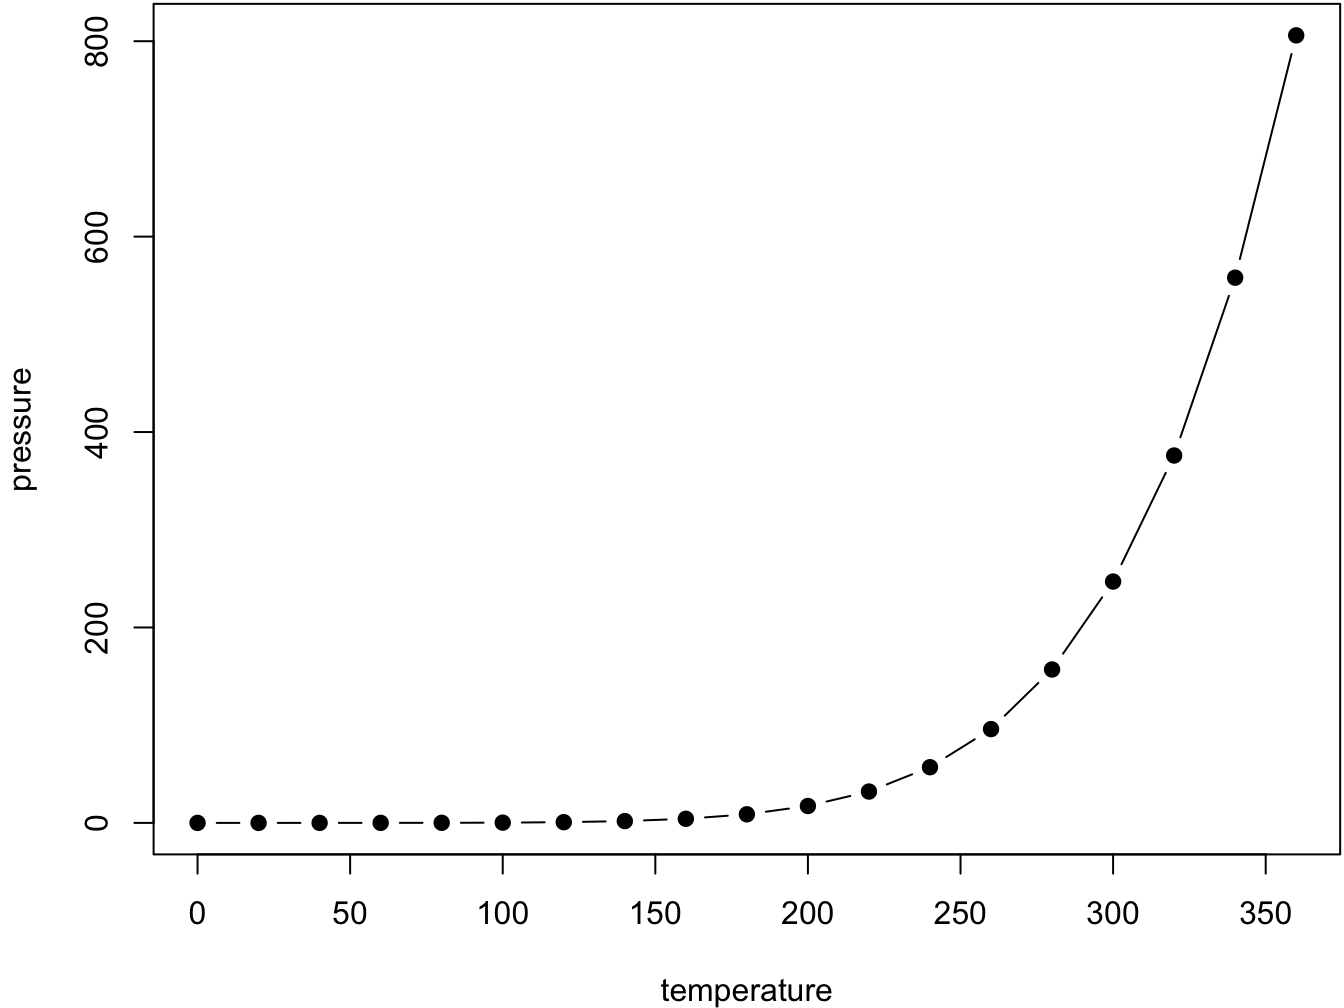
\includegraphics[width=0.8\linewidth]{bookdown-demo_files/figure-latex/nice-fig-1} 

}

\caption{Here is a nice figure!}\label{fig:nice-fig}
\end{figure}

Reference a figure by its code chunk label with the \texttt{fig:}
prefix, e.g., see Figure \ref{fig:nice-fig}. Similarly, you can
reference tables generated from \texttt{knitr::kable()}, e.g., see Table
\ref{tab:nice-tab}.

\begin{Shaded}
\begin{Highlighting}[]
\NormalTok{knitr}\OperatorTok{::}\KeywordTok{kable}\NormalTok{(}
  \KeywordTok{head}\NormalTok{(iris, }\DecValTok{20}\NormalTok{), }\DataTypeTok{caption =} \StringTok{'Here is a nice table!'}\NormalTok{,}
  \DataTypeTok{booktabs =} \OtherTok{TRUE}
\NormalTok{)}
\end{Highlighting}
\end{Shaded}

\begin{table}

\caption{\label{tab:nice-tab}Here is a nice table!}
\centering
\begin{tabular}[t]{rrrrl}
\toprule
Sepal.Length & Sepal.Width & Petal.Length & Petal.Width & Species\\
\midrule
5.1 & 3.5 & 1.4 & 0.2 & setosa\\
4.9 & 3.0 & 1.4 & 0.2 & setosa\\
4.7 & 3.2 & 1.3 & 0.2 & setosa\\
4.6 & 3.1 & 1.5 & 0.2 & setosa\\
5.0 & 3.6 & 1.4 & 0.2 & setosa\\
\addlinespace
5.4 & 3.9 & 1.7 & 0.4 & setosa\\
4.6 & 3.4 & 1.4 & 0.3 & setosa\\
5.0 & 3.4 & 1.5 & 0.2 & setosa\\
4.4 & 2.9 & 1.4 & 0.2 & setosa\\
4.9 & 3.1 & 1.5 & 0.1 & setosa\\
\addlinespace
5.4 & 3.7 & 1.5 & 0.2 & setosa\\
4.8 & 3.4 & 1.6 & 0.2 & setosa\\
4.8 & 3.0 & 1.4 & 0.1 & setosa\\
4.3 & 3.0 & 1.1 & 0.1 & setosa\\
5.8 & 4.0 & 1.2 & 0.2 & setosa\\
\addlinespace
5.7 & 4.4 & 1.5 & 0.4 & setosa\\
5.4 & 3.9 & 1.3 & 0.4 & setosa\\
5.1 & 3.5 & 1.4 & 0.3 & setosa\\
5.7 & 3.8 & 1.7 & 0.3 & setosa\\
5.1 & 3.8 & 1.5 & 0.3 & setosa\\
\bottomrule
\end{tabular}
\end{table}

You can write citations, too. For example, we are using the
\textbf{bookdown} package \citep{R-bookdown} in this sample book, which
was built on top of R Markdown and \textbf{knitr} \citep{xie2015}.

\hypertarget{chapter-format}{%
\section{Chapter Format}\label{chapter-format}}

\begin{itemize}
\tightlist
\item
  Claims from Fellowship
\end{itemize}

\hypertarget{chapter-1}{%
\section{Chapter 1}\label{chapter-1}}

\begin{itemize}
\tightlist
\item
  Theoretical Background Rationale for Computational Musicology and
  cognitive psychology

  \begin{itemize}
  \tightlist
  \item
    One
  \item
    Two

    \begin{itemize}
    \tightlist
    \item
      One a
    \item
      Two b
    \end{itemize}
  \end{itemize}
\item
  Goal in mind is how people learn melodies
\item
  Factors thought to contribute to mmd
\item
  End with polymorphism
\end{itemize}

\hypertarget{chapter-2}{%
\section{Chapter 2}\label{chapter-2}}

\begin{itemize}
\tightlist
\item
  History of Aural Skills
\item
  Current State of Aural Skills
\item
  Approaches and Goals
\end{itemize}

\hypertarget{chapter-3}{%
\section{Chapter 3}\label{chapter-3}}

\begin{itemize}
\tightlist
\item
  Cognitive Abilities
\item
  WMC

  \begin{itemize}
  \tightlist
  \item
    Definition of Why WMC is related to this
  \item
    Can learn a lot about melodic dictation by looking at WMC literature
  \end{itemize}
\item
  Experiment

  \begin{itemize}
  \tightlist
  \item
    Guts
  \end{itemize}
\item
  Discussion and Implications

  \begin{itemize}
  \tightlist
  \item
    Future studies need to look at WMC
  \item
    Future verbal theoretical and computational models should involve
    capcity measures (limits)
  \end{itemize}
\end{itemize}

\hypertarget{chapter-4}{%
\section{Chapter 4}\label{chapter-4}}

\begin{itemize}
\tightlist
\item
  Computation Chapter
\item
  From computational linguistics and information theory comes music comp
\item
  All papers citing FANTASTIC
\item
  n-gram models and IDyOM
\end{itemize}

\hypertarget{chapter-5}{%
\section{Chapter 5}\label{chapter-5}}

\begin{itemize}
\tightlist
\item
  Hello, corpus
\item
  History of Corpus studies (outside of music)
\item
  Current state, limitations
\item
  Descriptive statistics of the corpus
\end{itemize}

\hypertarget{chapter-6}{%
\section{Chapter 6}\label{chapter-6}}

\begin{itemize}
\item
  Experiments I and II
\item
  Used mixed effects models to incorporate both individual and musical
  differences
\item
  Problems with scoring (edit distance stuff, plus Buonviri)
\item
  Computational model, how that informs thinking about it (reasons from
  Lewandowsky)
\end{itemize}

\hypertarget{experiments}{%
\chapter{Experiments}\label{experiments}}

\hypertarget{rationale-for-experiment}{%
\section{Rationale for Experiment}\label{rationale-for-experiment}}

\hypertarget{selection-of-melodies}{%
\section{Selection of Melodies}\label{selection-of-melodies}}

\begin{itemize}
\tightlist
\item
  Tonalness, Countour, Number of Pitches - Long 1997 Tonalness good
  predictor
\item
  Tonalness better than atonal (Frances 1958) Zenatti 1969 -- from Long
  1997
\item
  Taylor 1977 -- IC predicts when contour and lenght constant
\item
  Long 1997 -- IC affects information
\end{itemize}

\hypertarget{experiment-i-and-ii}{%
\section{Experiment I and II}\label{experiment-i-and-ii}}

\hypertarget{experiment-iii}{%
\section{Experiment III?}\label{experiment-iii}}

\hypertarget{limitations-1}{%
\section{Limitations}\label{limitations-1}}

\hypertarget{how-to-score}{%
\subsection{How to Score}\label{how-to-score}}

\hypertarget{reasons-for-making-everything-open-source}{%
\subsection{Reasons for making everything open
source}\label{reasons-for-making-everything-open-source}}

\hypertarget{summaries}{%
\section{Summaries}\label{summaries}}

\hypertarget{applications-to-pedagoges}{%
\subsection{Applications to Pedagoges}\label{applications-to-pedagoges}}

\hypertarget{conceptual-frameworks}{%
\subsection{Conceptual Frameworks}\label{conceptual-frameworks}}

\hypertarget{conclusions}{%
\section{Conclusions}\label{conclusions}}

\hypertarget{what-can-we-really-expect-of-undergrads}{%
\subsection{What can we really expect of
undergrads?}\label{what-can-we-really-expect-of-undergrads}}

\hypertarget{reference-log}{%
\chapter{Reference Log}\label{reference-log}}

\hypertarget{to-incorporate}{%
\section{To Incorporate}\label{to-incorporate}}

\begin{itemize}
\item
  \citep{margulisModelMelodicExpectation2005} -- Margulis Model
\item
  \citep{nicholsScoreOneJazz2018} -- Specialty jazz background helps in
  tasks, WMC
\item
  \citep{NASM201718HandbookPdf2018} -- Fix intext
\item
  \citep{schumann1860musikalische} -- Quote about why people should do
  ear training
\item
  \citep{smith1934solfege} -- Quote from K2001 about why people should
  do ear training
\item
  \citep{longRelationshipsPitchMemory1977} -- Musical Characteristics
  predict memory
\item
  \citep{taylorStrategiesMemoryShort1983} -- Great citation that lots of
  things change memory, even structural!
\item
  \citep{tallaricoStudyThreePhase1974} -- Long boring talk on STM, LTM
\item
  \citep{ouraConstructingRepresentationMelody1991a} -- Awful
  experimental design that says people use structual tones
\item
  \citep{buonviriExplorationUndergraduateMusic2014} -- Call for
  experimental, suggestions as to what factors might contribute, use of
  deductive reasoning, qualitative
\item
  \citep{buonviriEffectsPreparatorySinging2015} -- People need to focus
  right away, not establish, distractors
\item
  \citep{buonviriEffectsMusicNotation2015} -- Showing people visual
  music does not help much.
\item
  \citep{buonviriEffectsTwoListening2017} -- Listening helps with other
  things, no best strategy in terms of writing
\item
  \citep{buonviriMelodicDictationInstruction2015} -- Literature to say
  people are bad at teaching melodic dictation and we don't know a lot
  about it, also interesting stuff about what solfege systems people use
\item
  \citep{davidbutlerWhyGulfMusic1997a} -- Call for music educators to do
  aural skills research, notes problem with aural skills pedagogy in
  lack of direction, also nice Nicholas Cook quotes on point of theory
\item
  \citep{furbyEffectsPeerTutoring2016} -- music ed study with weird
  stats, has references to follow up on with advantages of pitch systems
  and people who reccomend things for sight singing
\item
  \citep{pembrookInterferenceTranscriptionProcess1986} -- Effects of
  melodies, also how people do it. Interesting that they too effect of
  melodies, but talka bout things in terms of notes and not in terms of
  information content. Thought ot have an experiment where the n-grams
  that are more common are easier to write down. Lots of good charts
  too.
\item
  \citep{paneyEffectDirectingAttention2016} -- It's not good if you tell
  people what to do when they are dictating, article has a lot of good
  review for dictation materials to add to the `toRead' folder.
\item
  \citep{fournierCognitiveStrategiesSightsinging2017a} -- Good
  references that people are awful at Aural Skills, Also suggestions
  that people are not that great at transfer, and some stuff to suggest
  academic abililty is intertwined in all of this. Good reference for
  when starting to talk about untangling the mess that is aural skills.
\item
  \citep[ 1995]{berzWorkingMemoryMusic} -- Add on a new module to the
  WMC model of baddel with music, presents some evidence for why this
  theoretically should be included, but actually takes examples of
  dictation. A lot of this article felt like things that i was
  reinventing\ldots{}not good.
\item
  \citep{atkinsonSomeThoughtsOnTrying} -- Proof some other people are
  starting to think in terms of pedagogical schemas
\item
\end{itemize}

\hypertarget{chapter-3-1}{%
\section{Chapter 3}\label{chapter-3-1}}

\begin{itemize}
\item
  \citep{cowanWorkingMemoryCapacity2005} -- This book will probably
  serve as cornerstone of chapter in terms of creating relevant
  literature in addition to EE course readings on WMC. Provides history
  of WMC models and notes how attention based model as opposed to
  Baddely loop might actually be better theoretical model for talking
  about fact that WMC could just be something related to attention if
  not that. Provides extensive listing on problems with chunking that
  are all relevant to music, but then also supports it. Shows that
  Miller 1956 is a generally bad citation, own author even says that in
  Miller 1989 (check and add) and says limit is probably about 4 (use
  Cowan 2001 for ctation find that). Lots of good ideas like how music
  is always serial recall, examples of how to model the process, great
  discussions on zooming out and categorical nature of music within span
  of WMC ideas.
\item
  \citep{ockelfordMusicModuleWorking2007} -- uses case of savant to
  argue bits of Berz WM Music Model
\end{itemize}

\bibliography{book.bib,packages.bib}


\end{document}
